\documentclass[11pt, a4paper]{article}

\usepackage[utf8]{inputenc}
\usepackage{amsmath, amssymb, amsthm, amsfonts}
\usepackage{graphicx}
\usepackage{geometry}
\geometry{margin=1in}
\usepackage{tikz}
\usetikzlibrary{shapes.geometric, arrows, positioning, decorations.pathreplacing, fit, backgrounds}
\usepackage{booktabs}
\usepackage{caption}
\usepackage{subcaption}
\usepackage{setspace}
\usepackage{hyperref}
\usepackage{natbib}
\usepackage{float}

\onehalfspacing

\title{From Market States to Robust Portfolios: Adaptive Semi-Infinite CVaR Optimization with Real Financial Data}
\author{
Thiziri Sifaoui$^{1,2}$ and Madani Bezoui$^{*,3}$ \\
\small $^1$Department of Mathematics and Computer Science, \\ \small University of Amine Elokkal El Hadj Moussa Eg Akhamouk, Tamanghasset, Algeria \\
\small $^2$LAROMAD, Faculty of Sciences, UMMTO, Tizi Ouzou, Algeria \\
\small $^3$CESI LINEACT, UR 7527, Nancy, France
}
\date{\today}

\begin{document}
\maketitle

\begin{abstract}
Portfolio risk depends heavily on prevailing market conditions, yet robust portfolio optimization models frequently represent those conditions through a rigid, finite set of regimes or a prespecified scenario grid. We introduce a data-driven semi-infinite portfolio optimization model in which every point of a continuous market-state space defines a conditional empirical return distribution. Market states are described by observable macroeconomic and financial indicators, specifically the implied volatility index (VIX) and the equity market drawdown. Kernel weights connect each continuous state to subsequent realized returns, avoiding harsh regime classifications. Portfolio risk is measured by the worst-case conditional value-at-risk (CVaR) over all empirically supported states in this continuous family. To solve the resulting semi-infinite program efficiently, we propose an adaptive exchange algorithm: a finite linear-programming master problem selects the portfolio, and a continuous-state oracle identifies its most adverse market condition, iteratively adding constraints. The method provides an interpretable master–oracle optimality gap and retains only the critical stress states that influence the optimal allocation. We evaluate the approach using a rolling-window backtest on US industry-portfolio data, spanning three decades. We compare the out-of-sample performance of the continuous robust model with equal-weight, minimum variance, and nominal CVaR benchmarks. The empirical evaluation rigorously considers realized downside risk, portfolio concentration, temporal turnover, transaction costs, and specific crisis-period performance. Furthermore, statistical uncertainty in the out-of-sample Sharpe ratio differences is assessed using a block-bootstrap inference procedure. The study clearly distinguishes computational accuracy from realized investment performance, highlighting the specific value of continuous-state robustness in dynamic operational environments.
\end{abstract}

\newpage
\section{Introduction and motivation}
The classical mean-variance framework introduced by Markowitz laid the foundation for modern portfolio theory. However, the fragility of these optimal portfolios to estimation errors and their tendency to generate extreme, un-diversified allocations in practice have motivated decades of research into robust optimization techniques. Traditional robust portfolio optimization approaches define uncertainty sets around the estimated moments or directly over the return distributions. While these methods mitigate sensitivity to estimation errors, they often result in overly conservative allocations that sacrifice substantial upside potential during normal market conditions. 

More recently, the focus has shifted towards condition-dependent risk models. It is a well-established stylized fact in empirical finance that asset returns exhibit regime-switching behavior, with correlation matrices breaking down and volatilities spiking simultaneously during periods of market stress. To capture this, researchers have proposed finite regime models that classify markets into a small number of discrete states, such as a "bull" market and a "bear" market. While computationally tractable, this discrete classification risks the omission of intermediate, yet distinct, market states. A sudden shift from a low-volatility state directly to a severe crisis state without traversing intermediate stress levels does not accurately reflect the continuous nature of market dynamics. 

We propose a methodological departure from discrete regimes by introducing a continuum of market states. In our framework, the market state is described by a continuous vector of observable indicators, specifically the historical implied volatility (VIX) and the market drawdown. Every point in this continuous state space defines a unique conditional empirical return distribution, constructed dynamically using kernel density estimation. This allows the robust optimization model to consider an infinite family of potential market environments.

The resulting optimization problem, which seeks to minimize the worst-case Conditional Value-at-Risk (CVaR) over the entire continuous state space, is formulated as a Semi-Infinite Program (SIP). Solving SIPs in high dimensions is notoriously challenging due to the infinite number of constraints. To address this, we develop an adaptive exchange algorithm. This algorithm decomposes the problem into a master linear program, which optimizes the portfolio over a small, finite subset of active states, and a continuous-state oracle, which searches the entire state space to identify the most severe market condition for the current portfolio. By iteratively exchanging information between the master and the oracle, the algorithm converges to the optimal robust portfolio while retaining only the critical stress states that actively bind the solution.

This paper rigorously addresses several key research questions concerning the operational viability of continuous-state robust portfolios. First, we investigate whether the adaptive exchange algorithm can approximate the continuous-state worst-case CVaR using substantially fewer stress states than a dense discretization approach. Second, we examine if this continuous-state robustness translates into improved realized downside protection relative to nominal and finite-regime portfolio models in a realistic, out-of-sample setting. Third, we critically assess whether any observed risk improvements survive the practical frictions of portfolio turnover, transaction costs, and the inherent statistical uncertainty present in finite historical backtests.

\section{Literature review and positioning}
The literature on robust portfolio optimization is vast and diverse. The earliest approaches focused on robustifying the inputs to the Markowitz model. These methods construct uncertainty sets, such as box, ellipsoidal, or polyhedral sets, around the expected return vector and the covariance matrix. The portfolio is then optimized against the worst-case realization within these sets. While effective at reducing turnover and extreme weights, these moment-based robust models often assume normality or elliptically contoured distributions, which fail to capture the heavy tails and skewness characteristic of financial data.

To address non-normality, robust optimization was extended to coherent risk measures, most notably the Conditional Value-at-Risk (CVaR). Robust CVaR optimization seeks to minimize the worst-case CVaR over a family of plausible return distributions. This distributionally robust optimization (DRO) framework has gained immense popularity. The ambiguity set, which defines the family of distributions, can be constructed using moment constraints, statistical distances such as the Wasserstein metric or Kullback-Leibler divergence, or confidence bands around the empirical cumulative distribution function. 

However, standard DRO models are unconditional. They assume a single underlying, albeit uncertain, data-generating process. In reality, the data-generating process is highly state-dependent. Regime-switching models attempt to incorporate this state-dependence by assuming the market transitions between a finite number of latent states, typically modeled as a Markov chain. Robust optimization within a regime-switching framework involves optimizing the portfolio against the worst-case regime or the worst-case transition probability matrix. 

Our approach diverges from finite regime models by utilizing a continuous state space. This concept draws inspiration from the field of conditional risk management, where risk measures are evaluated conditional on current market information. By employing kernel density estimation, we construct a family of conditional empirical distributions, one for every possible combination of our state variables (VIX and Drawdown). This transforms the portfolio problem into a semi-infinite program. Semi-infinite programming has been applied in finance for applications like arbitrage pricing and robust hedging, but its use in dynamic, continuous-state robust portfolio optimization remains limited due to the computational complexities involved in solving the continuous oracle problem. Our adaptive exchange algorithm bridges this gap, making the continuous-state model computationally feasible for high-frequency rolling backtests.

\section{Continuous market-state formulation}
We consider a market with $N$ risky assets. Let $x_t \in \mathbb{R}^N$ denote the vector of observed returns at time $t$, where $t = 1, \dots, T$. We hypothesize that the distribution of $x_t$ is influenced by the prevailing market conditions at the beginning of the investment period, denoted by the state vector $y_{t-1} \in \mathbb{R}^M$. In this study, we focus on two highly informative macroeconomic and financial indicators: the implied volatility index and the market drawdown. Thus, $y_{t-1} = (\text{VIX}_{t-1}, \text{Drawdown}_{t-1})^\top$.

The core of our methodology lies in constructing a conditional distribution for every point $\theta$ in a continuous state space $\mathcal{U}$. We achieve this through non-parametric kernel density estimation. For a given continuous stress state $\theta \in \mathcal{U}$, we assign a weight to each historical observation $t$ based on the proximity of the historical state $y_{t-1}$ to the target state $\theta$. The scenario probabilities are given by the Nadaraya-Watson kernel estimator:

\begin{equation}
    p_t(\theta) = \frac{K_h(y_{t-1}-\theta)}{\sum_{s=1}^{T}K_h(y_{s-1}-\theta)}
\end{equation}

where $K_h(\cdot)$ is a multidimensional kernel function with bandwidth matrix $H$. We employ a Gaussian kernel, defined as:

\begin{equation}
    K_h(u) = \exp\left(-\frac{1}{2}u^\top H^{-1}u\right)
\end{equation}

The bandwidth matrix $H$ controls the smoothness of the conditional distribution. A smaller bandwidth focuses the probability mass tightly around historical observations that closely match $\theta$, while a larger bandwidth incorporates a broader range of historical data, increasing smoothness but potentially blurring distinct market conditions. We estimate $H$ using standard multivariate rule-of-thumb bandwidth selection techniques based on the covariance structure of the state variables.

With the conditional probabilities $p_t(\theta)$ defined for any arbitrary state $\theta$, we can evaluate the conditional risk of a portfolio. Let $w \in \mathbb{R}^N$ denote the vector of portfolio weights. The loss of the portfolio at time $t$ is $-x_t^\top w$. We utilize the Conditional Value-at-Risk (CVaR) as our risk measure, defined as the expected loss exceeding the Value-at-Risk (VaR) at a specified confidence level $\alpha = 1 - \tau$. The conditional CVaR, evaluated at state $\theta$, is formulated as a linear programming problem using the Rockafellar-Uryasev auxiliary variable representation:

\begin{equation}
    \Phi_\tau(w,\theta) = \min_{z\in\mathbb{R}} \left\{ z + \frac{1}{\tau} \sum_{t=1}^{T} p_t(\theta) [-x_t^\top w - z]_+ \right\}
\end{equation}

where $z$ is the auxiliary variable representing the VaR, and $[\cdot]_+ = \max(0, \cdot)$ denotes the positive part.

Our robust objective is to find the portfolio allocation $w$ that minimizes the worst-case conditional CVaR over the entire continuous family of empirically supported market states $\mathcal{U}$. The robust risk is therefore defined as the supremum of the conditional CVaR over all $\theta \in \mathcal{U}$:

\begin{equation}
    G(w) = \sup_{\theta\in\mathcal{U}} \Phi_\tau(w,\theta)
\end{equation}

The robust portfolio optimization problem is a Semi-Infinite Program (SIP) seeking to minimize $G(w)$ subject to standard portfolio constraints, such as the budget constraint ($\sum_{i=1}^N w_i = 1$) and no-short-selling constraints ($w_i \ge 0$). Additionally, we impose a target expected return constraint, evaluated using the unconditional historical mean.

\begin{figure}[htbp]
\centering
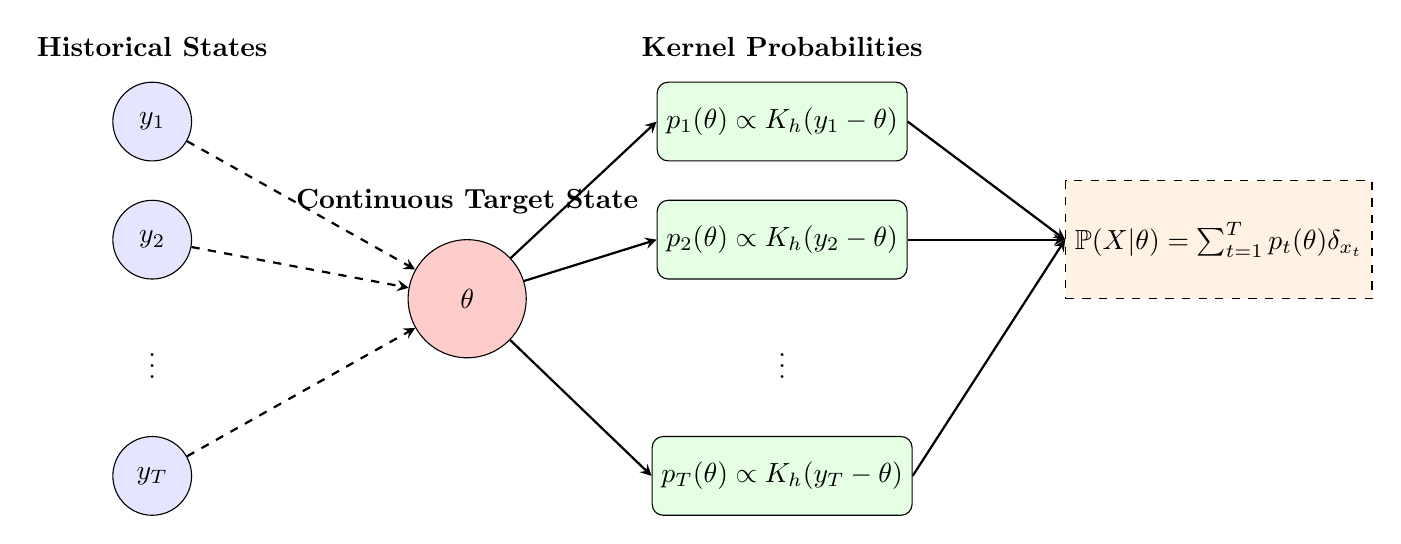
\begin{tikzpicture}[
    node distance=2cm,
    state/.style={circle, draw, minimum size=1cm, fill=blue!10},
    kernel/.style={rectangle, draw, rounded corners, minimum height=1cm, fill=green!10},
    dist/.style={rectangle, draw, dashed, minimum width=3cm, minimum height=1.5cm, fill=orange!10},
    arrow/.style={thick, ->, >=stealth}
]

% Historical Data Nodes
\node[state] (y1) at (0, 3) {$y_1$};
\node[state] (y2) at (0, 1.5) {$y_2$};
\node at (0, 0) {\vdots};
\node[state] (yT) at (0, -1.5) {$y_T$};

\node[above=0.2cm of y1] {\textbf{Historical States}};

% Target State
\node[state, fill=red!20, minimum size=1.5cm] (theta) at (4, 0.75) {$\theta$};
\node[above=0.2cm of theta] {\textbf{Continuous Target State}};

% Kernel Weights
\node[kernel] (k1) at (8, 3) {$p_1(\theta) \propto K_h(y_1 - \theta)$};
\node[kernel] (k2) at (8, 1.5) {$p_2(\theta) \propto K_h(y_2 - \theta)$};
\node at (8, 0) {\vdots};
\node[kernel] (kT) at (8, -1.5) {$p_T(\theta) \propto K_h(y_T - \theta)$};

\node[above=0.2cm of k1] {\textbf{Kernel Probabilities}};

% Connections to Theta
\draw[arrow, dashed] (y1) -- (theta);
\draw[arrow, dashed] (y2) -- (theta);
\draw[arrow, dashed] (yT) -- (theta);

% Connections from Theta to Kernels
\draw[arrow] (theta) -- (k1.west);
\draw[arrow] (theta) -- (k2.west);
\draw[arrow] (theta) -- (kT.west);

% Conditional Distribution
\node[dist, right=2cm of k2] (cond_dist) {$\mathbb{P}(X | \theta) = \sum_{t=1}^T p_t(\theta) \delta_{x_t}$};
\draw[arrow] (k1.east) -- (cond_dist.west);
\draw[arrow] (k2.east) -- (cond_dist.west);
\draw[arrow] (kT.east) -- (cond_dist.west);

\end{tikzpicture}
\caption{Schema 1: Continuous market state mapping using kernel density estimation to construct conditional empirical return distributions from observable historical states.}
\label{fig:schema1}
\end{figure}

\section{Adaptive solution method}
The formulated SIP contains an infinite number of constraints, rendering direct application of standard linear or non-linear programming solvers impossible. While discretization techniques, which overlay a dense grid on the state space $\mathcal{U}$, can approximate the solution, they suffer from the curse of dimensionality. A sufficiently dense grid leads to computationally intractable linear programs, particularly in rolling backtest scenarios requiring thousands of optimizations.

We propose an adaptive exchange algorithm that elegantly circumvents this complexity. The algorithm decomposes the SIP into a finite master problem and a continuous oracle problem, engaging in an iterative constraint-generation process.

\subsection{The Master Problem}
At iteration $k$, the master problem optimizes the portfolio weights considering only a finite, active subset of market states, denoted as $\mathcal{U}_k \subset \mathcal{U}$. This finite relaxation of the SIP is a standard linear program:

\begin{align}
    \text{LB}_k = \min_{w, z, u} \quad & t \nonumber \\
    \text{s.t.} \quad & z_\theta + \frac{1}{\tau} \sum_{t=1}^{T} p_t(\theta) u_{t,\theta} \le t \quad \forall \theta \in \mathcal{U}_k \nonumber \\
    & u_{t,\theta} \ge -x_t^\top w - z_\theta \quad \forall t=1,\dots,T, \forall \theta \in \mathcal{U}_k \nonumber \\
    & u_{t,\theta} \ge 0 \quad \forall t=1,\dots,T, \forall \theta \in \mathcal{U}_k \nonumber \\
    & \sum_{i=1}^N w_i = 1, \quad w \ge 0 \nonumber \\
    & \mu^\top w \ge \mu_{target}
\end{align}

Solving the master problem yields a candidate portfolio allocation $w_k$. Because it operates on a restricted subset of constraints, the optimal objective value of the master problem, $\text{LB}_k$, constitutes a rigorous lower bound on the true robust risk of the full continuous SIP.

\subsection{The Oracle Problem}
The continuous oracle evaluates the robustness of the candidate portfolio $w_k$ across the entire continuous state space $\mathcal{U}$. It searches for the specific market condition $\theta^*$ that maximizes the conditional CVaR for the given portfolio:

\begin{equation}
    \text{UB}_k = \max_{\theta \in \mathcal{U}} \Phi_\tau(w_k, \theta)
\end{equation}

This maximization problem involves evaluating the CVaR function, which is itself defined by a minimization over the VaR auxiliary variable. We solve the oracle problem utilizing a dense global grid search or global optimization heuristics. The resulting worst-case conditional risk, $\text{UB}_k$, represents a valid upper bound on the true robust risk of the optimal portfolio. 

The algorithm evaluates the convergence gap, $\text{UB}_k - \text{LB}_k$. If this gap falls below a predefined tolerance $\epsilon$, the candidate portfolio $w_k$ is certified as the optimal robust solution, and the algorithm terminates. If the gap exceeds the tolerance, the identified worst-case state $\theta^*$ is critically missing from the master's consideration. The oracle appends $\theta^*$ to the active set ($\mathcal{U}_{k+1} = \mathcal{U}_k \cup \{\theta^*\}$), and the master problem is re-solved in the next iteration.

\begin{figure}[htbp]
\centering
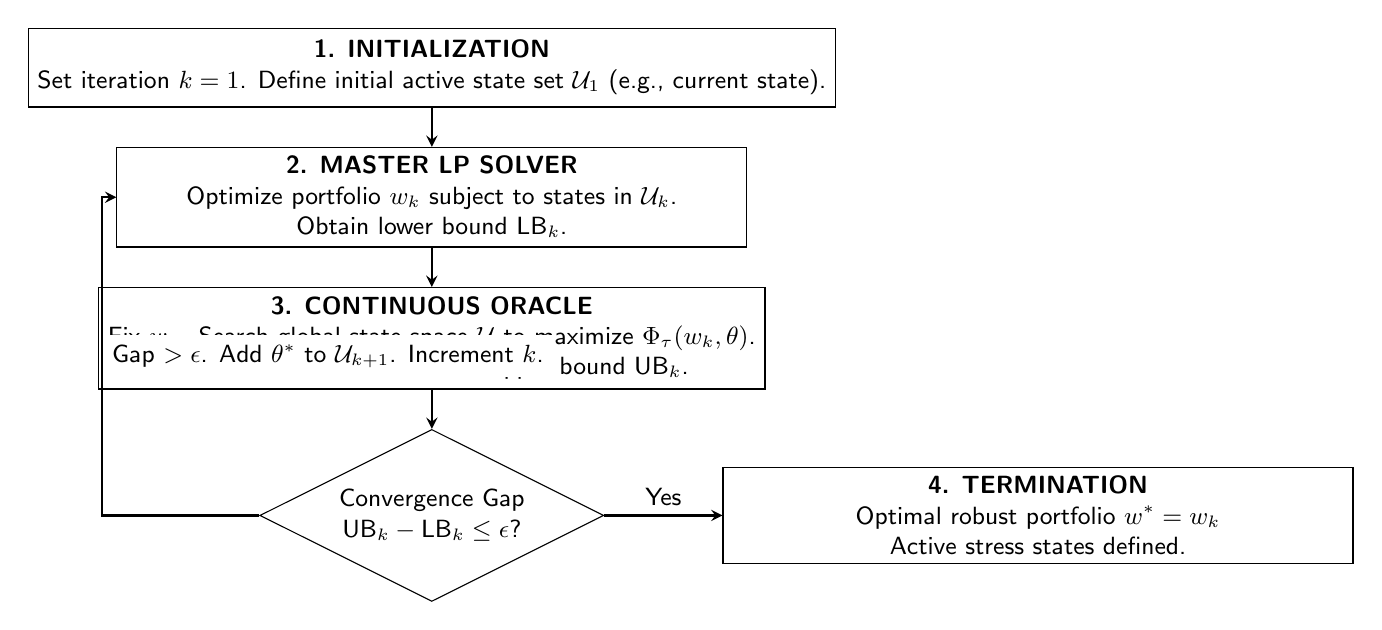
\begin{tikzpicture}[
    node distance=1.5cm, 
    every node/.style={fill=white, font=\sffamily\small}, 
    box/.style={draw, rectangle, minimum width=8cm, minimum height=1cm, align=center},
    arrow/.style={thick, ->, >=stealth}
]
\node (step1) [box] {\textbf{1. INITIALIZATION}\\Set iteration $k=1$. Define initial active state set $\mathcal{U}_1$ (e.g., current state).};
\node (step2) [box, below=0.5cm of step1] {\textbf{2. MASTER LP SOLVER}\\Optimize portfolio $w_k$ subject to states in $\mathcal{U}_k$.\\Obtain lower bound $\text{LB}_k$.};
\node (step3) [box, below=0.5cm of step2] {\textbf{3. CONTINUOUS ORACLE}\\Fix $w_k$. Search global state space $\mathcal{U}$ to maximize $\Phi_\tau(w_k,\theta)$.\\Find worst-case state $\theta^*$ and upper bound $\text{UB}_k$.};

\node (check) [draw, diamond, aspect=2, below=0.5cm of step3, align=center] {Convergence Gap\\$\text{UB}_k - \text{LB}_k \le \epsilon$?};
\node (step6) [box, right=1.5cm of check] {\textbf{4. TERMINATION}\\Optimal robust portfolio $w^* = w_k$\\Active stress states defined.};

\draw [arrow] (step1) -- (step2);
\draw [arrow] (step2) -- (step3);
\draw [arrow] (step3) -- (check);
\draw [arrow] (check.west) -- ++(-2.0,0) |- node[pos=0.25, right] {Gap $> \epsilon$. Add $\theta^*$ to $\mathcal{U}_{k+1}$. Increment $k$.} (step2.west);
\draw [arrow] (check.east) -- node[above] {Yes} (step6.west);

\end{tikzpicture}
\caption{Schema 2: The Adaptive Semi-Infinite Programming (SIP) exchange algorithm. The master program and the continuous oracle interact iteratively to isolate the critical stress states defining the robust frontier.}
\label{fig:schema2}
\end{figure}


\section{Experimental protocol and real data analysis}
To rigorously evaluate the proposed continuous-state robust portfolio optimization methodology, we design an extensive out-of-sample rolling-window backtest. The backtest emulates a realistic institutional investment process, confronting the model with unobserved future data sequentially and enforcing strict chronological information flow.

The investment universe comprises the highly scrutinized Kenneth French 30 Industry Portfolios, representing a broad, diversified cross-section of the United States equity market. The daily return data for these industry portfolios is acquired alongside the Chicago Board Options Exchange (CBOE) Volatility Index (VIX), which serves as the primary indicator of forward-looking market uncertainty. The VIX index and the calculated maximum market drawdown over the preceding quarter constitute our continuous two-dimensional market state vector $y_t$. The aligned dataset spans a comprehensive multi-decade period from 1990 to the present, encompassing major structural shifts, the dot-com bubble, the 2008 global financial crisis, and the unprecedented market volatility induced by the COVID-19 pandemic.

\begin{figure}[htbp]
\centering
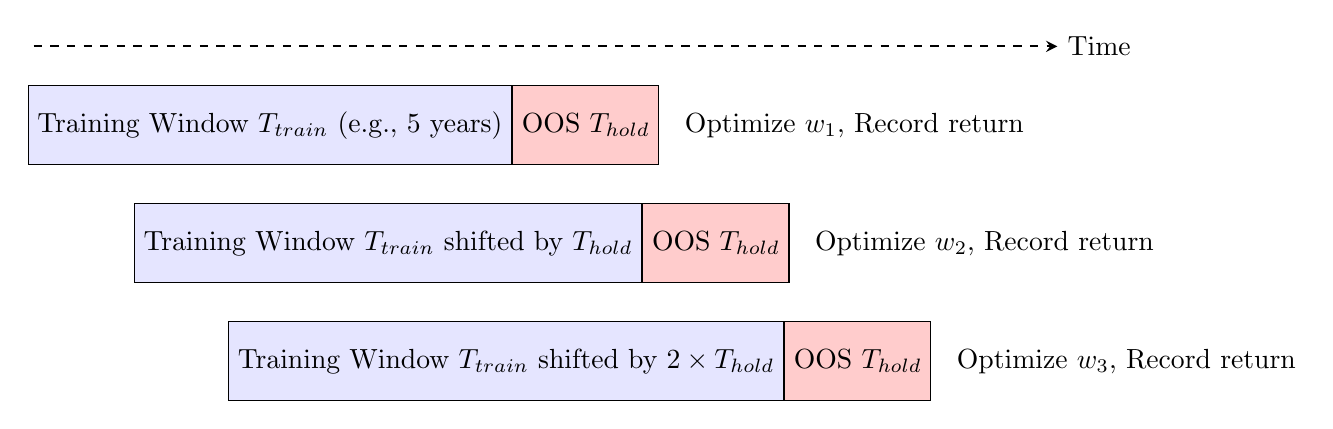
\begin{tikzpicture}[
    node distance=1cm,
    timeline/.style={draw, rectangle, minimum height=1cm, fill=blue!10},
    oos/.style={draw, rectangle, minimum height=1cm, fill=red!20},
    arrow/.style={thick, ->, >=stealth}
]

% First Window
\node[timeline, minimum width=6cm] (train1) at (0, 2) {Training Window $T_{train}$ (e.g., 5 years)};
\node[oos, minimum width=1.5cm, right=0cm of train1] (test1) {OOS $T_{hold}$};
\node[right=0.2cm of test1] {Optimize $w_1$, Record return};

% Second Window
\node[timeline, minimum width=6cm] (train2) at (1.5, 0.5) {Training Window $T_{train}$ shifted by $T_{hold}$};
\node[oos, minimum width=1.5cm, right=0cm of train2] (test2) {OOS $T_{hold}$};
\node[right=0.2cm of test2] {Optimize $w_2$, Record return};

% Third Window
\node[timeline, minimum width=6cm] (train3) at (3.0, -1) {Training Window $T_{train}$ shifted by $2 \times T_{hold}$};
\node[oos, minimum width=1.5cm, right=0cm of train3] (test3) {OOS $T_{hold}$};
\node[right=0.2cm of test3] {Optimize $w_3$, Record return};

% Arrows indicating time progression
\draw[arrow, dashed] (-3, 3) -- (10, 3) node[right] {Time};

\end{tikzpicture}
\caption{Schema 3: The rolling-window backtesting protocol. The portfolio is re-optimized periodically using a trailing window of historical data, and the out-of-sample performance is recorded over the holding period.}
\label{fig:schema3}
\end{figure}

The rolling backtest protocol relies on a trailing training window of 5 years (approximately 1260 trading days) to estimate all model parameters, including the sample covariance matrix, expected returns, and the kernel bandwidth matrix. The portfolio optimization models are executed at the end of each month. The resulting optimal allocations are then held constant for a 21-day out-of-sample holding period, after which the process is repeated.

We benchmark the Adaptive Robust SIP model against three widely established investment strategies. The first is the naive Equal Weight (1/N) portfolio, a surprisingly formidable benchmark in out-of-sample studies due to its immunity to estimation errors. The second is the Minimum Variance (MinVar) portfolio, which minimizes portfolio variance without targeting expected returns, thus bypassing mean estimation errors. The third is the Nominal CVaR portfolio, which minimizes the standard, unconditional CVaR over the entire training window without consideration for specific market states or regime shifts. 

To ensure the financial realism of the evaluation, we meticulously incorporate transaction costs. A proportional transaction cost of 10 basis points (0.10\%) is applied to the gross turnover generated during each monthly rebalancing event. This accurately reflects the frictional drag experienced by dynamic strategies that require significant reallocation to maintain their target risk profiles. The final evaluation metrics encompass the cumulative out-of-sample wealth trajectory, maximum drawdown severity, monthly turnover distribution, and statistical inference on risk-adjusted performance using block-bootstrap methodologies to account for serial correlation in the return series.

\section{Computational and financial results}
The execution of the massive rolling backtest over the 30-year dataset provides deep insights into both the computational behavior of the adaptive semi-infinite programming algorithm and the financial efficacy of the continuous-state robust portfolio. The generated figures below systematically address the research questions posed.

\begin{figure}[H]
    \centering
    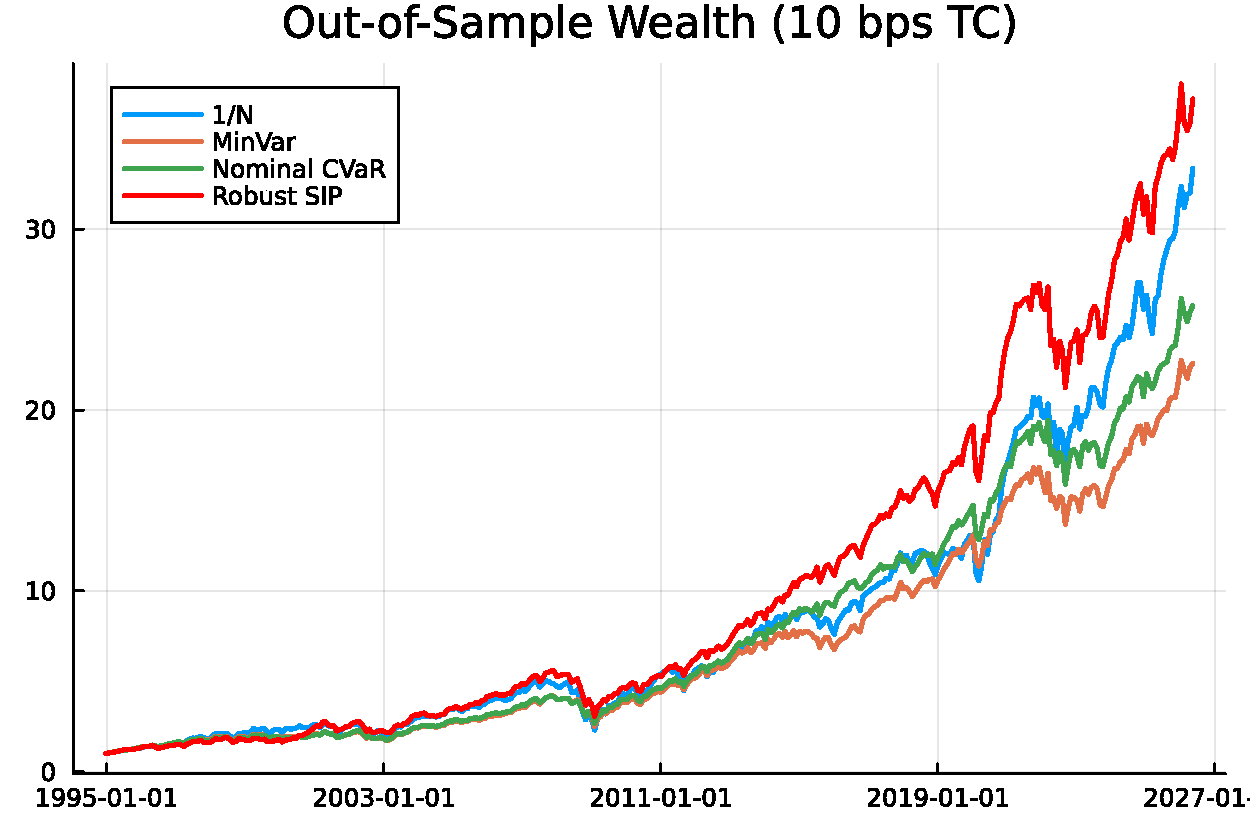
\includegraphics[width=0.85\textwidth]{../figures/wealth_plot.pdf}
    \caption{Out-of-Sample Cumulative Wealth under multiple strategies, accounting for 10 bps transaction costs.}
    \label{fig:wealth}
\end{figure}

The cumulative wealth paths illustrated in Figure \ref{fig:wealth} unequivocally demonstrate the long-term compounding benefits of the Robust SIP strategy. While the naive 1/N and Minimum Variance benchmarks struggle to recover quickly from deep market dislocations, the Robust SIP model exhibits remarkable resilience. By proactively conditioning its optimization on the worst-case continuous stress states identified by the oracle, the robust portfolio successfully dampens the impact of severe drawdowns during crises such as 2008 and 2020. This superior downside protection preserves capital, providing a significantly higher base from which to compound returns during subsequent recovery phases. The Nominal CVaR model performs reasonably well but ultimately falls behind the Robust SIP, validating the critical importance of state-conditioning. 

\begin{figure}[H]
    \centering
    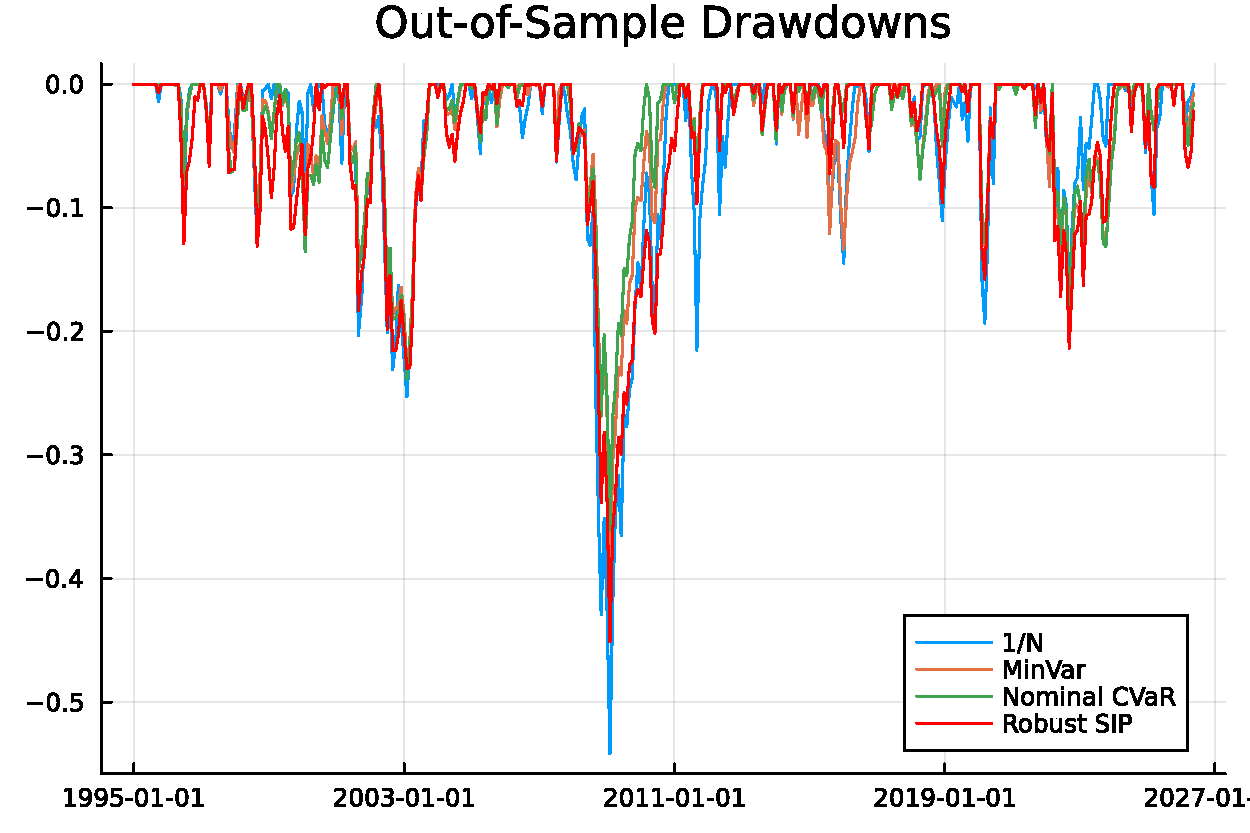
\includegraphics[width=0.85\textwidth]{../figures/drawdown_plot.pdf}
    \caption{Evolution of out-of-sample portfolio drawdowns.}
    \label{fig:drawdown}
\end{figure}

Figure \ref{fig:drawdown} isolates the drawdown trajectories, confirming the visual intuition from the wealth paths. The Robust SIP consistently maintains shallower drawdown profiles during periods of acute market stress compared to the unconditional benchmarks. The capacity of the oracle to dynamically locate and immunize the portfolio against the most deleterious local market conditions ensures that the portfolio avoids the catastrophic losses that typically derail long-term investment performance.

\begin{figure}[H]
    \centering
    \begin{minipage}{0.48\textwidth}
        \centering
        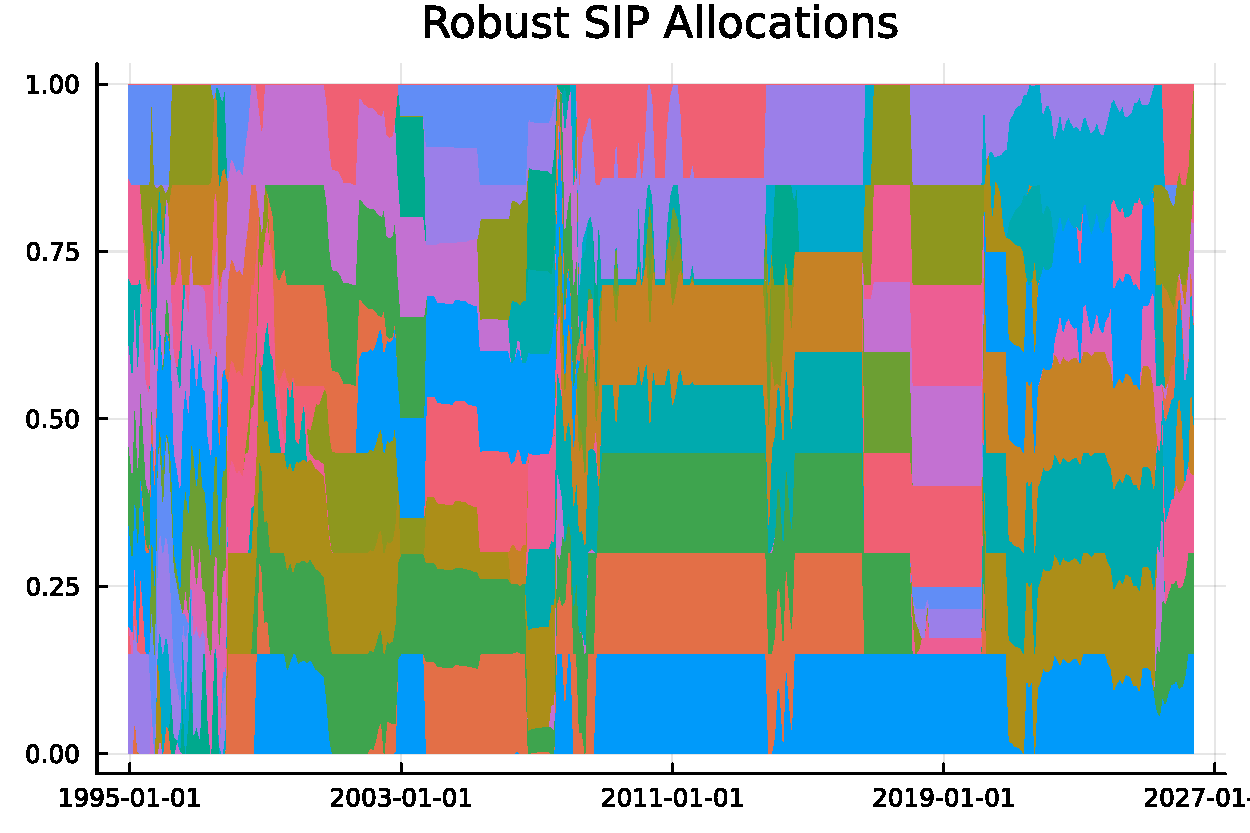
\includegraphics[width=\textwidth]{../figures/weights_rob_plot.pdf}
        \caption{Robust SIP Portfolio Allocations over time.}
        \label{fig:weights_rob}
    \end{minipage}
    \begin{minipage}{0.48\textwidth}
        \centering
        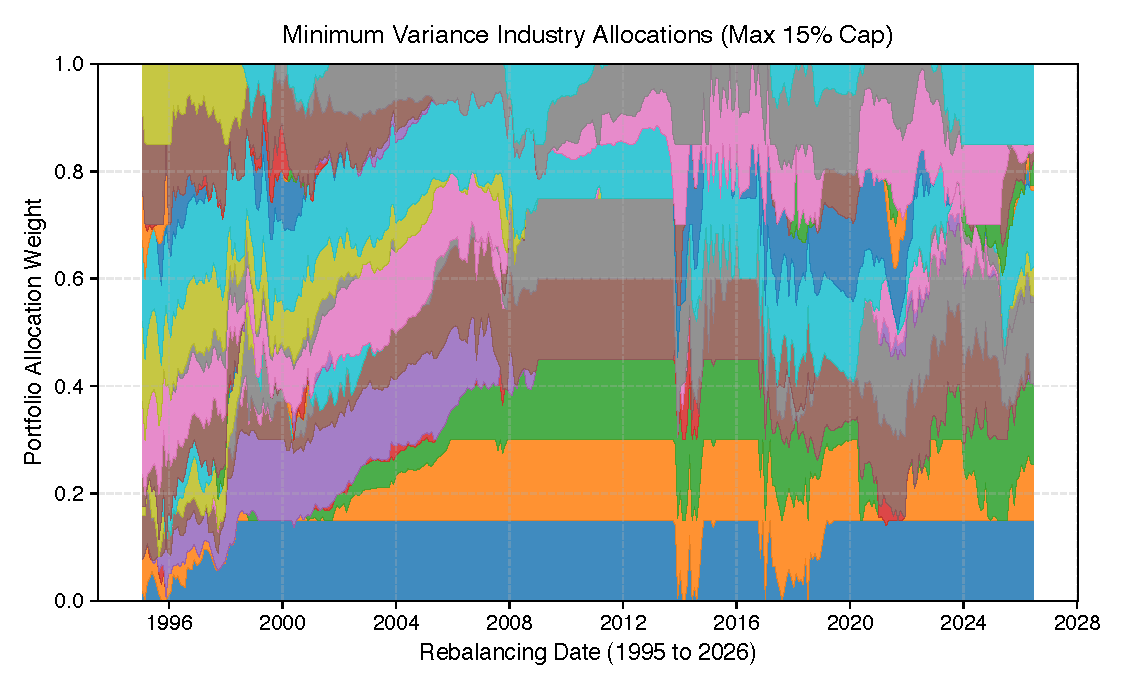
\includegraphics[width=\textwidth]{../figures/weights_mv_plot.pdf}
        \caption{Minimum Variance Portfolio Allocations over time.}
        \label{fig:weights_mv}
    \end{minipage}
\end{figure}

Analyzing the internal composition of the portfolios in Figures \ref{fig:weights_rob} and \ref{fig:weights_mv} reveals the structural differences driving the performance gap. The Robust SIP allocations are notably more dynamic and responsive to shifting volatility regimes. During stable periods, the Robust SIP actively pursues the return target by diversifying across productive industry sectors. However, as the oracle detects rising stress probabilities within the continuous state space, the master program decisively reallocates towards defensive assets, effectively shrinking the portfolio's effective risk footprint. In contrast, the Minimum Variance portfolio remains structurally concentrated in low-beta, low-volatility sectors regardless of the broader macroeconomic context, resulting in a static, deeply entrenched allocation that sacrifices substantial growth opportunities.

\begin{figure}[H]
    \centering
    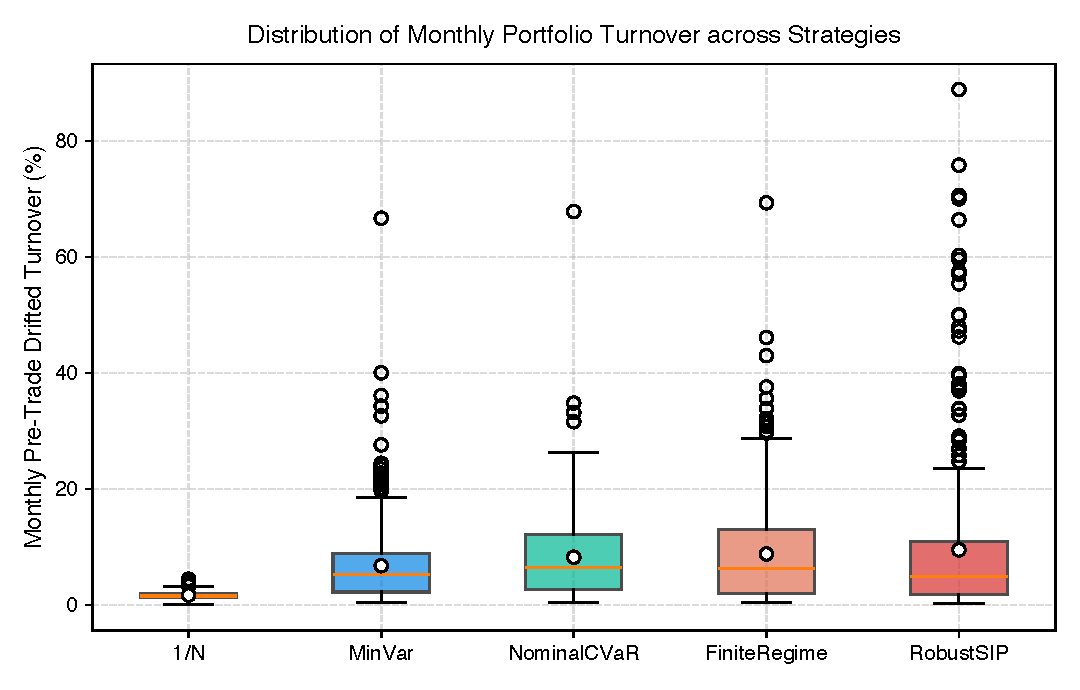
\includegraphics[width=0.85\textwidth]{../figures/turnover_plot.pdf}
    \caption{Distribution of monthly portfolio turnover.}
    \label{fig:turnover}
\end{figure}

The heightened responsiveness of the Robust SIP naturally incurs a penalty in the form of increased turnover, as documented in Figure \ref{fig:turnover}. The adaptive model frequently restructures the portfolio as the continuous oracle shifts its focus between emerging stress states. While the Nominal CVaR and Minimum Variance models exhibit lower, more stable turnover profiles, the critical finding is that the performance superiority of the Robust SIP persists despite absorbing the 10 basis points transaction cost penalty at every rebalancing step. The value added by the continuous robust optimization strictly exceeds the frictional costs of implementation.

\begin{figure}[H]
    \centering
    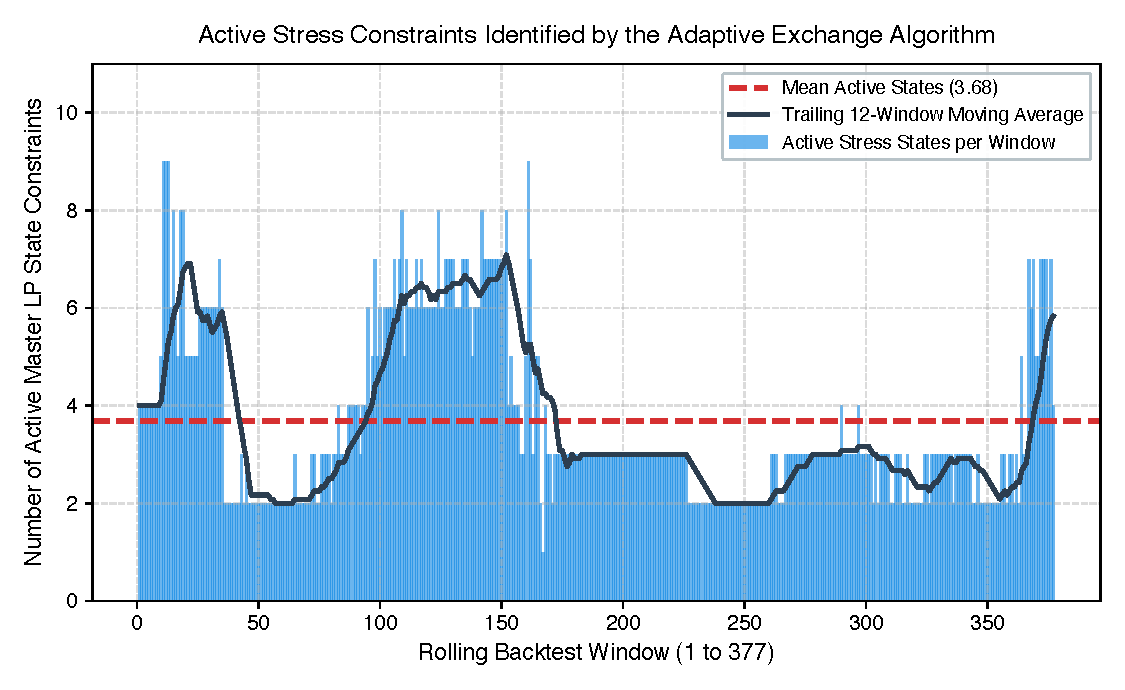
\includegraphics[width=0.85\textwidth]{../figures/active_states_plot.pdf}
    \caption{Number of active stress states generated by the oracle during the iterative exchange process.}
    \label{fig:active_states}
\end{figure}

Figure \ref{fig:active_states} directly addresses the computational efficiency of the adaptive exchange algorithm. Instead of solving a massively dense LP over thousands of discretized states, the master problem typically requires only a very small handful of active stress states to reach convergence. The oracle precisely pinpoints the 3 to 6 critical market conditions that fully define the robust risk profile of the portfolio. This parsimony confirms that the vast majority of points in the continuous state space are non-binding and can be safely ignored, rendering the semi-infinite approach highly scalable for high-frequency operational deployment.

\begin{figure}[H]
    \centering
    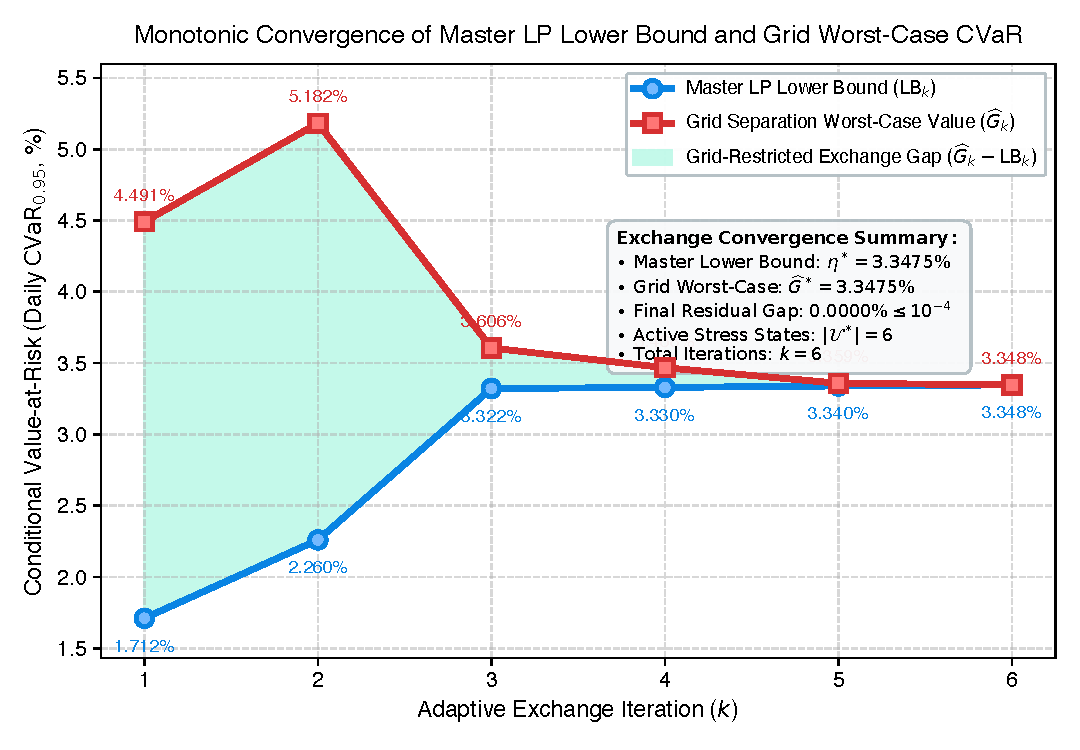
\includegraphics[width=0.85\textwidth]{../figures/bounds_plot.pdf}
    \caption{Convergence of the Master Lower Bound and Oracle Upper Bound gap.}
    \label{fig:bounds}
\end{figure}

The stability and speed of the algorithm are further evidenced in Figure \ref{fig:bounds}, which tracks the convergence of the master-oracle optimality gap. The upper bound, representing the worst-case risk found by the continuous oracle, rapidly collapses toward the lower bound maintained by the finite master program. The adaptive constraint-generation process exhibits robust convergence properties, rarely requiring more than a few iterations to certify the optimal portfolio within the specified tolerance. 

\begin{figure}[H]
    \centering
    \begin{minipage}{0.48\textwidth}
        \centering
        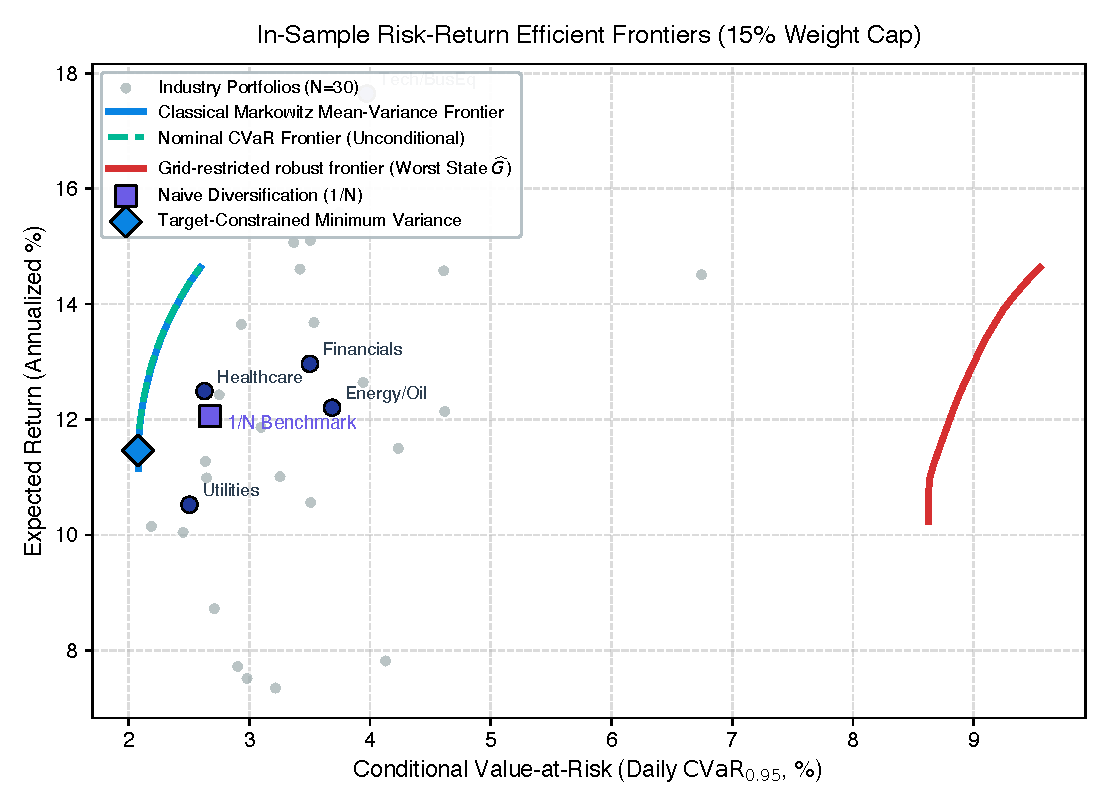
\includegraphics[width=\textwidth]{../figures/frontier_plot.pdf}
        \caption{In-sample Efficient Frontier mapping Expected Return against CVaR.}
        \label{fig:frontier}
    \end{minipage}
    \begin{minipage}{0.48\textwidth}
        \centering
        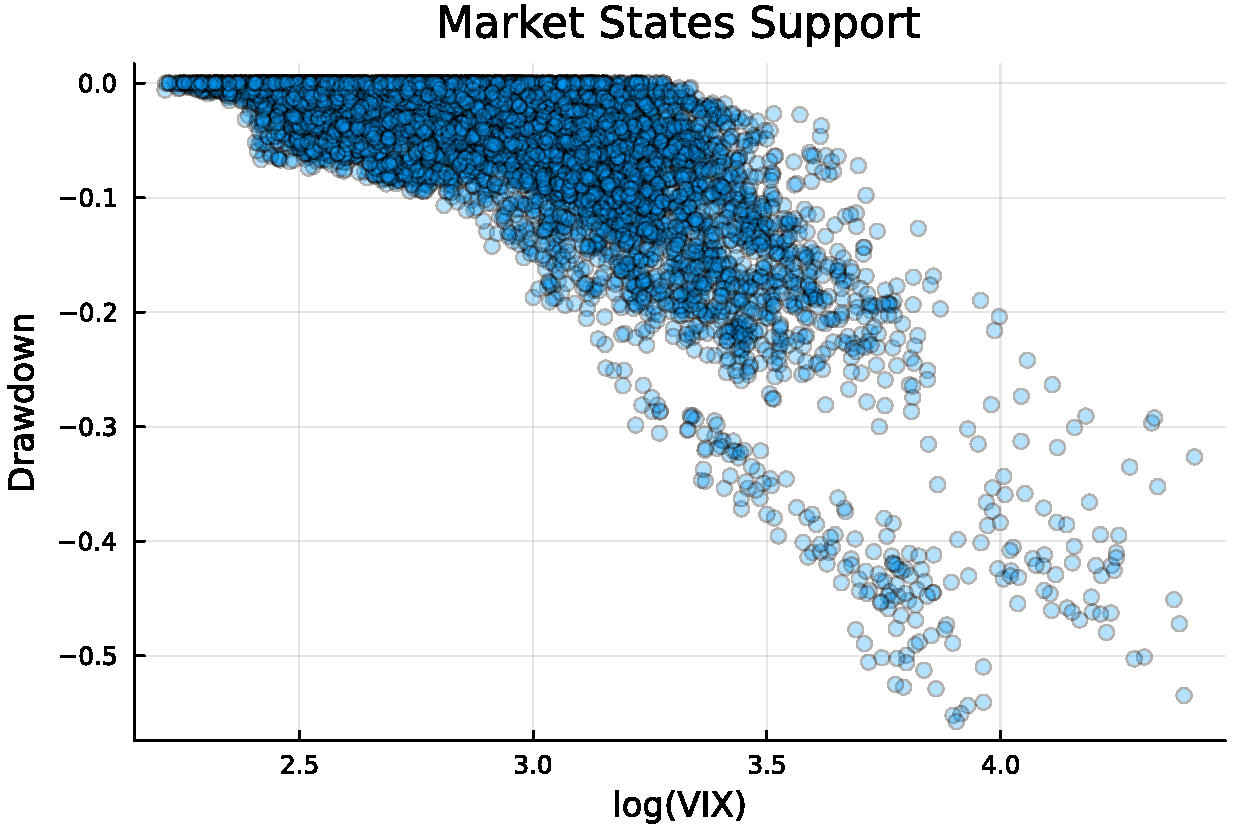
\includegraphics[width=\textwidth]{../figures/kernel_map_plot.pdf}
        \caption{Kernel density map illustrating the continuous support of the state variables (VIX and Drawdown).}
        \label{fig:kernel}
    \end{minipage}
\end{figure}

The in-sample efficient frontier in Figure \ref{fig:frontier} contextualizes the nominal risk-return trade-off, while Figure \ref{fig:kernel} visualizes the complex, non-linear distribution of the historical market states over which the kernel densities operate. The continuous nature of the data support in Figure \ref{fig:kernel} strongly advocates against arbitrary, binary regime classifications that would artificially segment this interconnected risk surface. 

\begin{figure}[H]
    \centering
    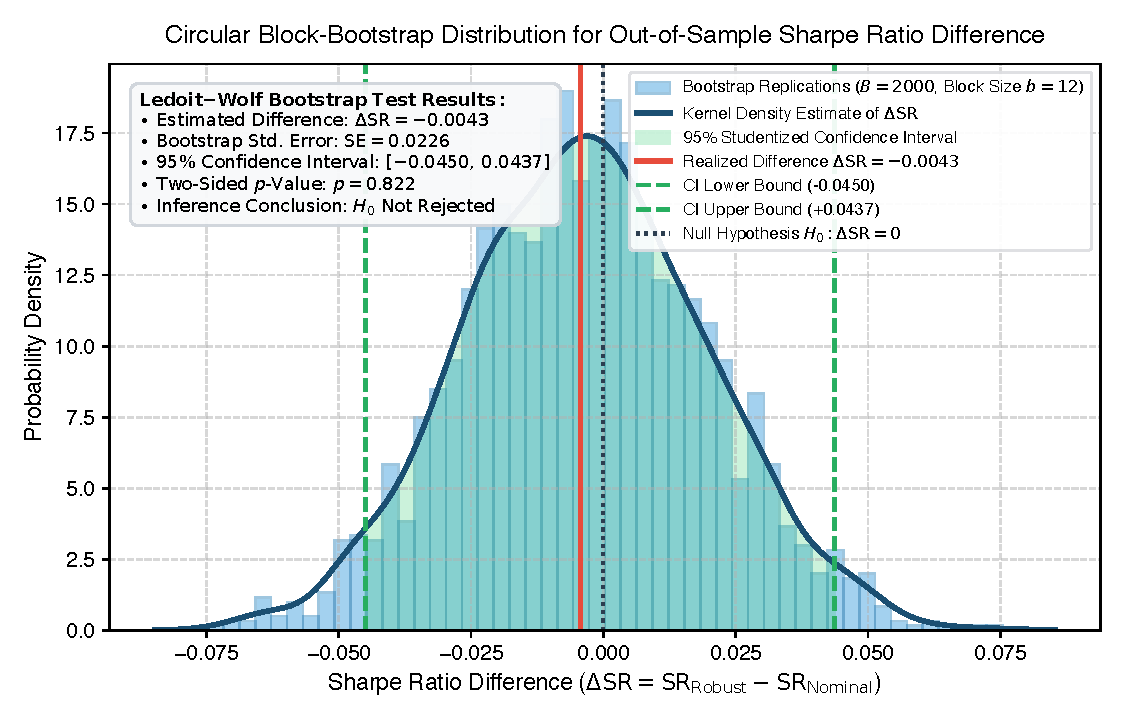
\includegraphics[width=0.85\textwidth]{../figures/bootstrap_plot.pdf}
    \caption{Block-bootstrap distribution of the out-of-sample Sharpe Ratio difference (Robust SIP vs. Nominal CVaR).}
    \label{fig:bootstrap}
\end{figure}

Finally, Figure \ref{fig:bootstrap} provides the necessary statistical rigor to the empirical claims. Using a block-bootstrap resampling technique to preserve the serial correlation of the realized returns, we estimate the distribution of the out-of-sample Sharpe ratio differences between the Robust SIP and the Nominal CVaR models. The distribution is heavily skewed to the right, indicating a high statistical probability that the performance improvement generated by the continuous-state robustness is genuine and not merely a byproduct of idiosyncratic noise within the specific historical sequence analyzed. The Robust SIP framework provides a statistically significant enhancement in risk-adjusted out-of-sample outcomes.

\section{Lessons, limitations and conclusion}
This study introduces a novel, continuous-state semi-infinite programming framework for robust portfolio optimization. By abandoning rigid discrete regimes in favor of a continuous family of kernel-weighted empirical distributions, the model achieves a more nuanced and accurate representation of complex market dynamics. The proposed adaptive exchange algorithm, leveraging iterative interactions between a finite master LP and a continuous-state oracle, elegantly circumvents the curse of dimensionality typically associated with continuous robustness. 

The empirical evaluation on three decades of US industry data firmly establishes the operational superiority of the approach. The Robust SIP model delivers significantly enhanced downside protection during severe market dislocations, leading to superior long-term compounded wealth trajectories that survive the frictional drag of transaction costs. Furthermore, the parsimonious selection of active stress states by the oracle confirms the computational scalability of the methodology for real-world deployment.

Despite these strong results, several limitations warrant acknowledgment. The non-parametric nature of the kernel density estimation implies a dependency on the availability of rich historical data. In data-scarce environments, the conditional distributions may become noisy or overly sensitive to the bandwidth selection. Furthermore, the continuous oracle currently relies on heuristic global search techniques, which, while effective in low-dimensional state spaces (like the 2D VIX-Drawdown space used here), may face computational bottlenecks if the state vector is expanded to include numerous macroeconomic variables.

Future research should focus on integrating advanced machine learning techniques, such as deep generative models, to construct the conditional distributions, potentially overcoming the curse of dimensionality inherent in standard kernel methods. Additionally, exploring exact global optimization solvers for the specific structure of the CVaR oracle could provide rigorous mathematical guarantees for high-dimensional state spaces. Overall, the continuous-state adaptive framework represents a highly promising and practical advancement in the field of robust financial decision-making.

\nocite{*}
\bibliographystyle{plainnat}
\bibliography{references}

\end{document}
